\documentclass[12pt]{article}
\usepackage{hyperref}
\usepackage[fleqn]{amsmath}
\usepackage{amsfonts}
\usepackage{float}
\usepackage{amsthm}
\usepackage{graphicx}

\usepackage{tikz}

\newcommand*{\aut}{\mathcal{A}}
\newcommand*{\Int}{\mathbb{Z}}
\newcommand*{\myvec}[1]{\vec{#1}}
\newcommand{\cefaout}{\mathcal{O}}
\newcommand{\Lang}{\mathcal{L}}
\newcommand{\arrconcat}{\sharp}
\newcommand{\denghang}[1]{{\color{teal}\textbf{DH:} #1 \textbf{:HD}\color{black}}}
\newcommand{\comment}[1]{{\color{blue}\textbf{MARK:} #1 \textbf{:KRAM}\color{black}}}
\newcommand{\todo}[1]{{\color{orange}\textbf{TODO:} #1 \textbf{:ODOT}\color{black}}}
\newcommand{\mysplit}{\mathsf{split}}
\newcommand{\myjoin}{\mathsf{join}}
\newcommand{\mylen}{\mathsf{len}}
\newcommand{\myread}{\mathsf{read}}
\newcommand{\mywrite}{\mathsf{write}}
\newcommand{\myset}[1]{\{#1\}}


\theoremstyle{remark}
\newtheorem{definition}{Defination}[section]

\title{A Note for Solving String Constraints with Split Function}
\author{Denghang Hu}
\begin{document}
\maketitle

\section{Preliminary}
\subsection{Cost-enriched Finite State Automata (CEFA)}
In this section, we define the cost-enriched finite state automata (CEFA), which was introduced in \cite{atva2020} and will be used to solve the satisfiability problem of RECL later on. 
%
Intuitively, CEFA adds write-only cost registers to finite state automata. ``write-only'' means that the cost registers can only be written/updated but cannot be read, i.e., they cannot be used to guard the transitions. 

%
%In~\cite{atva2020}, the cost function is defined as a function $\eta: \Sigma \rightarrow \mathbb{N}$. In this paper, we define the cost function as an integer vector whose elements are the incremental value of registers. Furthermore, we add a new linear integer arithmetic constraint $\theta$ to each final state of the CEFA, which restricts the value of registers. Two types of definitions have the same expressive ability on the $SAT_{CL}$ problem.
\vspace{-0.5mm}
\begin{definition}[Cost-Enriched Finite Automaton]
    A cost-enriched finite automaton $\aut$ is a tuple $(R, Q, \Sigma, \delta, I, F, \alpha)$ where
    \begin{itemize}
        \item $R = \{r_1, \cdots, r_k\}$ is a finite set of registers,
        \item $Q, \Sigma, I, F$ are as in the definition of NFA,
              %    \item $R = (r_1\cdots r_n)$ is a vector of mutually distinct cost registers,
        \item $\delta \subseteq Q \times \Sigma \times Q \times \Int^R$ is a transition relation, where $\Int^R$ denotes the updates on the values of registers.
              %  set whose elements are tuples $(q, c, q', \myvec{v})$ where $q, q'$ are states of $Q$, $c$ is a letter in alphabet $\Sigma\cup\{\epsilon\}$ and $\myvec{v}$ is the cost update function for registers, which is an integer vector whose $i$-th element is the incremental value of register $r_i$.  $(q, a, q', \myvec{v})$ is written as $q\xrightarrow[\myvec{v}]{a} q'$ for readability.
        \item $\alpha \in \Phi(R)$ is an LIA formula specifying an accepting condition.
              %    a linear integer arithmetic constraint function on final states. $\theta$ is called \emph{accepting condition}.
    \end{itemize}
\end{definition}
\vspace{-0.5mm}

For convenience, we use $R_\aut$ to denote the set of registers of $\aut$. We assume a linear order on $R$ and write $R$ as a vector $(r_1, \cdots, r_k)$. Accordingly, we write an element of $\Int^R$ as a vector $(v_1, \cdots, v_k)$, where $v_i$ is the update of $r_i$ for each $i \in [k]$. We also write a transition $(q, a, q', \vec{v}) \in \delta$ as $q \xrightarrow[\vec{v}]{a} q'$. The transition $(q,a,q',())$ with empty updates is abbreviated as $(q,a,q')$.
%The definition of CEFA above is slightly different from the definition in~\cite{atva2020} in the sense that accepting conditions on register values
%are attached to final states. 

The semantics of CEFA is defined as follows. Let $\aut = (R, Q, \Sigma, \delta, I, F, \alpha)$ be a CEFA. 
%A \emph{configuration} of $\aut$ is a pair $(q, \vec{v})$ where $q \in Q$ and $\vec{v}$ is a vector denoting the values of registers.  
%An \emph{initial configuration} of $\aut$ is $(q_0, \vec{0})$ with $q_0 \in I$, where the value of each register is zero. 
A \emph{run} of $\aut$ on a string $w = a_1 \cdots a_n$ is a sequence $q_0 \xrightarrow[\myvec{v_1}]{a_1} q_1 \cdots q_{n-1}\xrightarrow[\myvec{v_n}]{a_n} q_n$ such that $q_0 \in I$ and $q_{i-1} \xrightarrow[\myvec{v_i}]{a_i} q_i$ for each $i \in [n]$. A run $q_0 \xrightarrow[\myvec{v_1}]{a_1} q_1 \cdots q_{n-1}\xrightarrow[\myvec{v_n}]{a_n} q_n$ is \emph{accepting} if $q_n \in F$ and $\alpha(\myvec{v'}/R)$ is true, where $\myvec{v'} = \sum \limits_{j \in [n]} \myvec{v_j}$. The vector $\myvec{v'}= \sum \limits_{j \in [n]} \myvec{v_j}$ is called the \emph{cost} of an accepting run $q_0 \xrightarrow[\myvec{v_1}]{a_1} q_1 \cdots q_{n-1}\xrightarrow[\myvec{v_n}]{a_n} q_n$. Note that the values of all registers are initiated to zero and updated to $\sum \limits_{j \in [n]} \myvec{v_j}$ after all the transitions in the run are executed. We use $\myvec{v'} \in \aut(w)$ to denote the fact that there is an accepting run of $\aut$ on $w$ whose cost is $\myvec{v'}$.  
We define the semantics of a CEFA $\aut$, denoted by $\Lang(\aut)$, as $\{(w; \myvec{v'}) \mid  \myvec{v'} \in \aut(w)\}$.  In particular, if $I \cap F \neq \emptyset$ and $\alpha(\myvec{0}/R)$ is true, then $(\varepsilon; \myvec{0}) \in \Lang(\aut)$. Moreover, we define the \emph{output} of a CEFA $\aut$, denoted by $\cefaout(\aut)$, as $\{\myvec{v'} \mid  \exists w.\ \myvec{v'} \in \aut(w)\}$.


\subsection{Special CEFA for String Array}
%%
We define a special CEFA for string array. The CEFA uses a preserved character $``\arrconcat"$ as $array$ elements separator (note that $\arrconcat\not\in\Sigma$). The speciality of $\aut_s$ rely on  its construction.
%%
\paragraph{Array of fixed length and constant index} Considering an $array$ $A$ with fixed length $m$, we assume that each array element $A[i]$ $(i\in[1,m])$ is constrained by a CEFA $\aut_i\equiv (R_i, Q_i, \Sigma, \delta_i, I_i, F_i, \alpha_i)$. Note that the index of the array starts from 1.  Then we can construct the CEFA of the array $A$ as $\aut_s\equiv (R_s, Q_s, \Sigma\cup\{\arrconcat\}, \delta_s, I_s, F_s, \alpha_s)$, where:
\begin{itemize}
    % \item $R_s = \bigcup\limits_{1\leq i \leq m} R_i$,
    \item $R_s = \bigcup\limits_{1\leq i \leq m} R_i\cup \myset{r}$ for a fresh register r,
    \item $Q_s = \bigcup\limits_{1\leq i \leq m} Q_i\cup \myset{q_0, q_f}$ for fresh states $q_0$ and $q_f$,
    \item $\delta_s$ is composed of four transitions set
          \begin{itemize}
              \item  $\{(q_0, \arrconcat, q_1, (\myvec{0}, 1))\mid q_1\in I_1\}$,
              \item  $\myset{(q_m, \sharp, q_f, (\myvec{0}, 0))\mid q_m\in F_m}$,
              \item  $\{(q, \arrconcat, q', (\myvec{0}, 1)) \mid q\in F_i, q'\in I_{i+1}, i\in[1,m]\}$ where $ I_{m+1}=\emptyset$,
              \item  and $\{(q, a, q', (\myvec{0},\myvec{v_i},\myvec{0}))\mid (q, a, q', \myvec{v_i})\in \aut_i, i\in[1,m]\}$,
          \end{itemize}
          where $(\myvec{0}, 1)$ is a vector that increases the value of $r$ by 1 and remains other registers unchanged, and $(\myvec{0},\myvec{v_i},\myvec{0})$ is a vector that updates the value of $R_i$ by $\myvec{v_i}$ and remains other registers unchanged. Similarly for $(\myvec{0}, 0)$ and so on.
    \item $I_s = \myset{q_0}$, $F_s = \myset{q_f},$ and $\alpha_s = \bigwedge\limits_{1\leq i \leq m} \alpha_i$.
          % and $\alpha_s = \bigwedge\limits_{1\leq i \leq m} \alpha_i$.
\end{itemize}
The resulting CEFA is shown in fig \ref{fig:fixed_len_cons_idx}, where $q_i\in I_i$ and $q_i'\in F_i$ for each $i\in [1,m]$. The main idea of the construction above is using $\arrconcat$ to separate each element of the array and one register to record the index of each element. We introduce two fresh states $q_0$ and $q_f$ to ensure each element is started and ended with at least one $\arrconcat $, which is beneficial to the construction of pre-images of string constraints (see \ref*{sec:pre_image} for more details). The accepting condition $\alpha_s$ is the conjunction of accepting conditions of each element.
% It is obviously that the accepting word $w$ of $\aut_s$ is in language $\mathcal{L}(\aut_1)\arrconcat\mathcal{L}(\aut_2)\ ... \ \arrconcat \mathcal{L}(\aut_{m}) $.
\begin{figure}[H]
    \centering
    \usetikzlibrary {automata, positioning, fit}
    \begin{tikzpicture}[initial text =, initial distance=3ex,
            node distance=1.2cm, auto,
            state/.style={circle, draw, inner sep=0pt, minimum size=5mm},
            accepting by double]
        
        \node[state,initial]            (q_0)                {$q_0$};
        \node[state]                    (q_1) [right=of q_0] {$q_1$};
        \node[state]                    (q_1') [right=of q_1] {$q_1'$};
        \node                           (omit)[right=of q_1'] {$\cdots$};
        \node[state]                    (q_m) [right=of omit] {$q_m$};
        \node[state]                    (q_m') [right=of q_m] {$q_m'$};
        \node[state, accepting]         (q_f)  [right=of q_m'] {$q_f$};
        
        \node[draw, fit=(q_1) (q_1'), inner sep=0.5em, label=above:$\aut_1$] [dashed] {};
        \node[draw, fit=(q_m) (q_m'), inner sep=0.5em, label=above:$\aut_m$] [dashed] {};
        
        \path[->]
        (q_0) edge [above] node {$\scriptstyle \arrconcat$} (q_1)
        (q_0) edge [below] node {${\scriptstyle r++}$} (q_1)
        (q_1') edge [above] node {$\scriptstyle \arrconcat$} (omit)
        (q_1') edge [below] node {${\scriptstyle r++}$} (omit)
        (omit) edge [above] node {$\scriptstyle \arrconcat$} (q_m)
        (omit) edge [below] node {${\scriptstyle r++}$} (q_m)
        (q_m') edge [above] node {$\scriptstyle \arrconcat$} (q_f)
        (q_m') edge [below] node {${\scriptstyle r}$} (q_f);
        
    \end{tikzpicture}
    \caption{The CEFA of $A$ with accepting condition $\alpha_s = \bigwedge\limits_{1\leq i \leq m} \alpha_i$}
    \label{fig:fixed_len_cons_idx}
\end{figure}
The construction of $\aut_s$ can be used to formalize the array containing constant string. For example, for a 2-length array $A$ constrained by $``a" = \myread(A, 1)\wedge ``b" = \myread(A, 2) \wedge \mylen(A) = 2$ , where $\myread(A, m)$ read the  element of $A$ at constant index $m$ and $\mylen(A)$ is the length of $A$, we can construct the automaton of $A$ as following: \\
$(\emptyset, \{q_0,q_1,q_1',q_2,q_2'\}, \{a,b,\arrconcat\}, \{q_0\xrightarrow[(1)]{\arrconcat}q_1, q_1\xrightarrow[(0)]{a}q_1', q_1'\xrightarrow[(1)]{\arrconcat}q_2, q_2\xrightarrow[(0)]{b}q_2'\}, \{q_0\}, \{q_2'\}, \top)$. 
%%
\paragraph{Array of varible length and index} \todo{TODO}

\section{Straight-Line String Theory with Integer and Array $SL_{I,A,S} $}\label{sec:SL}
We defined a theory $SL_{I,A,S}$ with three sorts: \textbf{string}, \textbf{integer} and \textbf{array}. The \textit{elements} of \textbf{array} can only be \textbf{string} sort, and the $index$ of \textbf{array} is \textbf{Integer} sort.
\subsection{Syntax}
The syntax of $SL_{I,A,S}$ is defined in table \ref{tab:syntax} where: $e$ is a regular expression; $\mylen(A)$ is the length of array $A$, $\mylen(x)$ is the length of string $x$; $\myread(A, m)$ read the  element of $A$ at index $m$, $\mywrite(B, x ,m)$ write string $x$ to array $B$ at index $m$;  $\myjoin(A,u)$ connect all of elements in array $A$ by connector $u$; $\mysplit(s,e)$ split string $x$ into ordered string array by separator $e$; $y\cdot z$ connects string $y$ and $z$; $\circ \in \{=,\not=, <, \leq, >, \geq \}$ is the set of arithmatic binary predicates.
%  For technical convenience, we assume that all assignments in F are \textit{Static Singly Assignment (SSA)} form.
\begin{table}
    \renewcommand{\arraystretch}{1.5}
    \begin{tabular}{l l l r}
        $x,y$ & $\cdots$ &                                                                       & String varibles          \\
        $m,n$ & $\cdots$ &                                                                       & Integer constants        \\
        $i,j$ & $\cdots$ &                                                                       & Integer varibles         \\
        $A,B$ & $\cdots$ &                                                                       & Array varibles           \\
        $t$   & $::=$    & $m \mid i \mid t+t \mid t-t \mid \mylen(A)\mid \mylen(x) $            & Integer term             \\
        $SC$  & $::=$    & $x=\myread(A, m) \mid A = \mywrite(B, x ,m) \mid x=\myjoin(A,u) \mid$ &                          \\
              &          & $A = \mysplit(x, e) \mid x= y\cdot z\mid x\in e$                      & String constraints       \\
        $F$   & $::=$    & $t\circ t \mid SC \mid F\wedge F $                                    & Formula of $SL_{I,A,S} $

    \end{tabular}
    \caption{Syntax of $SL_{I,A,S}$}
    \label{tab:syntax}
\end{table}
\subsection{Defination of Straight-Line Restriction }
We consider two sorts: \textbf{string} and \textbf{array}.
\begin{definition}[Relational constraints ]
    Relational constraints $\phi$ are defined by the following rules:
    \begin{align*}
        \phi \ ::= \  & x=y\cdot z \mid x=\myjoin(A,u) \mid A = \mysplit(x,e) \mid        \\
                      & x=\myread(A, m) \mid A = \mywrite(B, x ,m) \mid \phi \wedge \phi 
    \end{align*}
\end{definition}
\begin{definition}[Straight-line relational constraints]
    A relational constraint $\phi$ is straight-line if $\phi = \bigwedge\limits_{1\leq i \leq m} \chi_i = P_i$ such that
    \begin{itemize}
        \item $\chi_1,\cdots,\chi_m $ are mutally distinct string varibles and array varibles.
        \item For each $i\in [m] $, all the varibles in $P_i$ are in the set $\{\chi_1,\cdots,\chi_{m-1} \}$.
    \end{itemize}
\end{definition}
\begin{definition}[Straight-line formula]
    A formula $F$ of $SL_{I,A,S}$ is straight-line iff all relational constraints in $F$ are straight-line.
\end{definition}
% \begin{figure}[H]
%     % denote
%     % $u,v,\cdots$  \hfill{String constants}\\
%     $x,y,\cdots$  \hfill{String varibles}\\
%     $m,n,\cdots$  \hfill{Integer constants}\\
%     $i,j,\cdots$  \hfill{Integer varibles}\\
%     % $M,N,\cdots$  \hfill{Array constants}\\
%     $A,B,\cdots$  \hfill{Array varibles}\\ 

%     % term and expression
%     % $s \ ::= \ u \mid x$ \hfill{String term}\\
%     $t \ ::= \  m \mid i \mid t+t \mid t-t \mid |A|\mid |x| $ \hfill{Integer term}\\
%     % $A \ ::= \  M \mid X  $ \hfill{Array term}\\
%     % $\beta \ ::= \  m \mid |A| \mid |A|+m  $  \hfill{Bound expression}\\

%     % formula
%     % $LA \ ::= \ t\circ t \mid LA\wedge LA \mid \neg LA $  \hfill{Linear arithmatic}\\
%     $SC \ ::= \ x=read(A, m) \mid A = write(A, x ,m) \mid x=\myjoin(A,u)\mid A = \mysplit(x, e) \mid x\in e$   \flushright{String constraints}\\
%     % $AC \ ::= \ A = \mysplit(s,e) \mid A = A[\beta_1:\beta_2] \mid A = A[t\rightarrow s] \mid A\in \aut_s \mid A = \mathcal{T}(A) $ \flushright{Array constraints}\\ 
%     $F \ ::= \ t\circ t \mid SC \mid F\wedge F $ \hfill{Formula of $SL_{I,A,S} $}
%     \caption{Syntax of $SL_{I,A,S}$}
%     \label{fig:syntax}
% \end{figure}

% \section{Pre-image of String Constraints}
% \subsection{Array Assignment}
% Assume $A\in \aut_s$ and $\aut_s=(Q, \Sigma, \delta,q_0,F,R)$ construct like fig \ref{fig:special_nfa}.
% \begin{itemize}
%     \item $A = \mysplit(s,e)$: assume $e\in \mathcal{A}_e$, then we can construct $\mathcal{B}=(Q', \Sigma', \delta',q_0,F,R)$ like fig \ref{fig:pre_image_split} s.t $s\in B$.
%     \item $B = A[\beta_1:\beta_2]$:
% \end{itemize}

% % \begin{itemize}
% %     \item $e$ : A regular expression.
% %     \item $A[m]$ : Return the $element$ of $A$ at index $m$.
% %     % \item $A[t\rightarrow s]$ : Return a new array the same as $A$ except  that the $element$ of $A$ at index $t$ changes to string $s$.
% %     % \item $s\cdot s$ : String concatenation.
% %     \item $\myjoin(A,u) $ : Return a new string by concatenating all of $elements$ in array $A$, separated by a specified separator string $u$.
% %     \item $\mysplit(s,e) $ : Return a new array by dividing string $s$ into ordered substring array. The separator string is regular expression $e$.
% %     % \item $\mathcal{T}(A) $: Return a new array by applying transducer $\mathcal{T}$ on each $element$ of array $A$.
% %     % \item $A[\beta_1:\beta_2] $ Return a new array which is the subarray of $A$.
% % \end{itemize}
% % \subsection{Defination of Straight-Line Restriction }
% We consider two sorts: \textbf{string} and \textbf{array}.
% \begin{definition}[Relational constraints ]
%     Relational constraints $\phi$ are defined by the following rules:
%     \begin{align*}
%         \phi \ ::= \ x=s\cdot s \mid x=\myjoin(A,u) \mid A = \mysplit(s,e) \mid A = A[\beta_1:\beta_2] \mid A = A[t\rightarrow s] \mid \phi \wedge \phi
%     \end{align*}
% \end{definition}
% \begin{definition}[Straight-line relational constraints]
%     A relational constraint $\phi$ is straight-line if $\phi = \bigwedge\limits_{1\leq i \leq m} x_i = P_i$ such that
%     \begin{itemize}
%         \item $x_1,\cdots,x_m $ are mutally distinct.
%         \item For each $i\in [m] $, all the varibles in $P_i$ are either source varibles or varibles in set $\{x_1,\cdots,x_{m-1} \}$.
%     \end{itemize}
% \end{definition}
% \begin{definition}[Straight-line formula]
%     A formula $F$ of $SL_{I,A,S}$ is straight-line iff all relational constraints in $F$ are straight-line.
% \end{definition}


% \begin{figure}
%     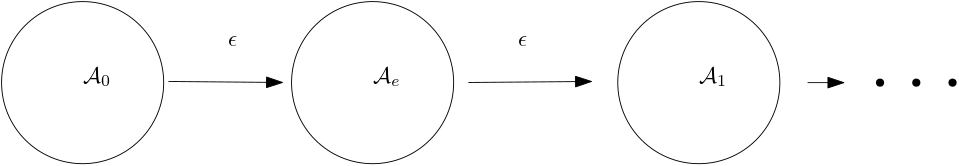
\includegraphics[width=\linewidth]{pre_image_split.png}
%     \caption{pre-image of split operation}
%     \label{fig:pre_image_split}
% \end{figure}
% \bibliographystyle{abbrv} % 指定格式,
% % \bibliographystyle{apa} % 这是姓名年份应用格式
% \bibliography{ref} %  ../.bib表示bib的具体位置

\section{Pre-images of String Constraints}\label{sec:pre_image}
In this section, we define the pre-image of each string constraint formula.
\paragraph{- $i = \mylen(A)$:} The pre-image for this formula is a CEFA $\aut_A=(R_A, Q_A, \Sigma\cup\{\arrconcat\}, \delta_A, I_A, F_A, \alpha_A)$, where
\begin{itemize}
    \item $R_A = \{r\}$ for a fresh register $r$, $Q_A = \{q_0, q_f\}$, $\delta_A = \myset{q_0\xrightarrow[(0)]{\Sigma}q_0, q_0\xrightarrow[(1)]{\sharp}q_0, q_0\xrightarrow[(0)]{\arrconcat}q_f }$, $I_A = \myset{q_0}$, $F_A = \myset{q_f}$, and $\alpha_A \equiv r = i$.
\end{itemize}

\paragraph{- $i = \mylen(x)$:} As the pre-image of length function in \cite{atva2020}.

\paragraph{- $x = \myread(A, m)$:} Suppose that $x$ is constrained by $\aut_x=(R_x, Q_x, \Sigma, \delta_x, I_x, F_x, \alpha_x)$, then the pre-image for $A$ is a CEFA $\aut_A=(R_A, Q_A, \Sigma\cup\{\arrconcat\}, \delta_A, I_A, F_A, \alpha_A)$, where
\begin{itemize}
    \item $R_A = R_x$,
    \item $Q_A = Q_x\cup\myset{q_0, q_1, \cdots, q_{m}}$,
    \item $\delta_A$ is the union of six transitions set:
          \begin{itemize}
              \item $\myset{q_i\xrightarrow[(\myvec{0})]{\Sigma}q_i\mid i\in [1,m-1]}$,
              \item $\myset{q_i\xrightarrow[(\myvec{0})]{\arrconcat}q_{i+1}\mid i\in[0,m-2]}$,
              \item $\myset{q_{m-1}\xrightarrow[(\myvec{0})]{\arrconcat}q_0^x \mid q_0^x\in I_x}$,
              \item $\myset{q_f^x\xrightarrow[(\myvec{0})]{\arrconcat}q_m \mid q_f^x\in F_x}$,
              \item $\myset{q_m\xrightarrow[(\myvec{0})]{\arrconcat}q_m}$,
              \item $\myset{q\xrightarrow[(\myvec{v})]{a}q'\mid q\xrightarrow[\myvec{v}]{a}q'\in \delta_x}$.
          \end{itemize}
    \item $I_A = \myset{q_0}$, $F_A = \myset{q_m}$, and $\alpha_A = \alpha_x$.
\end{itemize}

\paragraph{- $A = \mywrite(B, x, m)$:} Suppose that $A$ is constrained by $\aut_A=(R_A, Q_A, \Sigma\cup\{\arrconcat\}, \delta_A, I_A, F_A, \alpha_A)$, we firstly consider $A$ as a \emph{string varible} in the formula $A = x_1\arrconcat x_2\arrconcat x_3$. The pre-image of the formula is a set of tuple $(\aut_1, \aut_2, \aut_3)$ in which $x_1\in \aut_1, x_2\in \aut_2, x_3\in \aut_3$. There is at least one tuple with both $\aut_1$ and $\aut_3$ to be non-empty, as we ensure that each element of array is started and ended with at least one $\arrconcat$. Then the pre-image of $A = \mywrite(B, x, m)$ is a set of tuple $(\aut_B, \aut_x)$ where
\begin{itemize}
    \item $\aut_B = \aut_1'\arrconcat\Sigma^*\arrconcat\aut_3$, $\aut_1'$ add a new register $r$ to $\aut_1$ to record the occurence times of $\arrconcat$ in $\aut_1$ and add the constraint $r = m$ for the occurence times,
    \item $\aut_x = \aut_2$.
\end{itemize}

\paragraph{- $x = \myjoin(A,u)$:} Suppose that $x$ is constrained by $\aut_x=(R_x, Q_x, \Sigma, \delta_x, I_x, F_x, \alpha_x)$, then the pre-image is a CEFA

\end{document}